
%(BEGIN_QUESTION)
% Copyright 2012, Tony R. Kuphaldt, released under the Creative Commons Attribution License (v 1.0)
% This means you may do almost anything with this work of mine, so long as you give me proper credit

``Flare'' på et raffineri brukes for sikker avlastning av hydrokarbongasser ved forbrenning. Et ``knockout drum'' skiller væske fra damp slik at kun damp går til flare-tip. Oppsamlet væske dreneres til OWS:

$$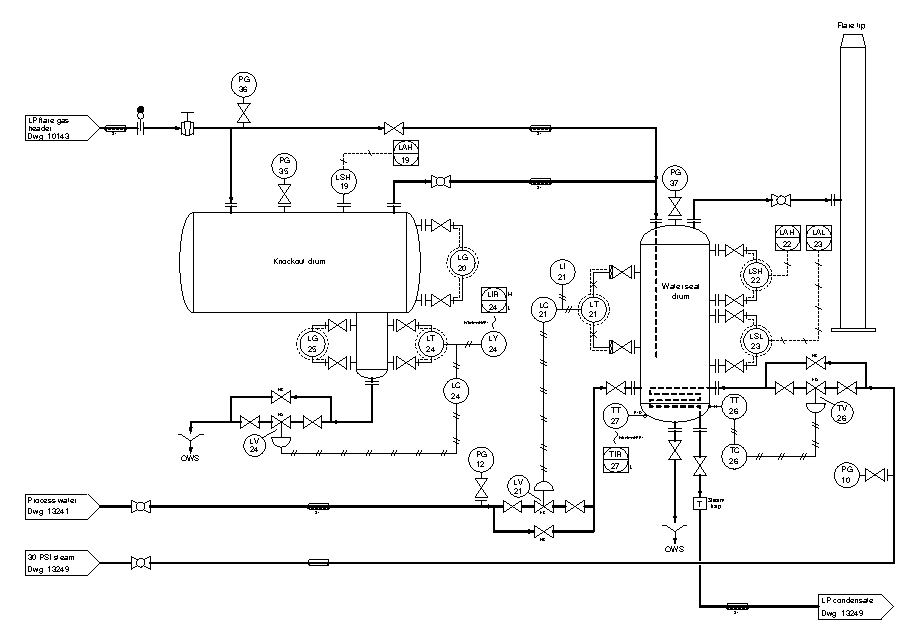
\includegraphics[width=15.5cm]{i0002rx01.eps}$$

Sammensetningen mot flare varierer kraftig. Drift ønsker å overvåke total flow av hydrokarbonmateriale som brennes. Ingeniører vurderer måleteknologi og plassering.

\vskip 10pt

Foreslå ulike flowteknologier og vurder om de passer her.

\underbar{file i00977}
%(END_QUESTION)





%(BEGIN_ANSWER)

Riktig plassering for dampmåler er mellom knockout drum og water-seal drum, eller mellom water-seal drum og flare-tip, med riktige rettstrekklengder.

\vskip 10pt

\begin{itemize}
\item{} {\bf Orifice/venturi} -- normalt lite egnet uten kompensering for tetthet, trykk og temperatur.
\vskip 10pt
\item{} {\bf Fortrengning} -- lite egnet (partikler, temperaturvariasjon, og risiko ved eventuell blokkering).
\vskip 10pt
\item{} {\bf Turbin} -- mulig, men krever P/T-kompensering.
\vskip 10pt
\item{} {\bf Vortex} -- ofte lite egnet pga. lavflow-cutoff.
\vskip 10pt
\item{} {\bf Magnetisk} -- uegnet for ikke-ledende gass.
\vskip 10pt
\item{} {\bf Ultralyd Doppler} -- uegnet uten reflektorer i strømmen.
\vskip 10pt
\item{} {\bf Ultralyd transit-time} -- mulig, med P/T-kompensering.
\vskip 10pt
\item{} {\bf Coriolis} -- teknisk egnet, men ofte kostbar.
\vskip 10pt
\item{} {\bf Termisk masse} -- uegnet ved ukjent/varierende spesifikk varme.
\end{itemize}

 
%(END_ANSWER)





%(BEGIN_NOTES)


%INDEX% Process: flare knockout drum and water seal (realistic P&ID shown)

%(END_NOTES)

